\documentclass[sigconf,anonymous]{acmart}

\usepackage{arydshln}
\usepackage{hyperref}
\usepackage{multirow}
\usepackage{geometry}
\usepackage{listings}
\usepackage{xcolor}
\usepackage{amsmath} 
\usepackage{amsfonts}

\lstdefinelanguage{json}{
    basicstyle=\small\ttfamily,
    numbers=left,
    numberstyle=\tiny,
    stepnumber=1,
    numbersep=8pt,
    showstringspaces=false,
    breaklines=true,
    frame=lines,
    backgroundcolor=\color{gray!10},
    literate=
     *{0}{{{\color{blue}0}}}{1}
      {1}{{{\color{blue}1}}}{1}
      {2}{{{\color{blue}2}}}{1}
      {3}{{{\color{blue}3}}}{1}
      {4}{{{\color{blue}4}}}{1}
      {5}{{{\color{blue}5}}}{1}
      {6}{{{\color{blue}6}}}{1}
      {7}{{{\color{blue}7}}}{1}
      {8}{{{\color{blue}8}}}{1}
      {9}{{{\color{blue}9}}}{1}
      {:}{{{\color{red}{:}}}}{1}
      {,}{{{\color{red}{,}}}}{1}
      {\{}{{{\color{purple}{\{}}}}{1}
      {\}}{{{\color{purple}{\}}}}}{1}
      {[}{{{\color{purple}{[}}}}{1}
      {]}{{{\color{purple}{]}}}}{1},
}

\AtBeginDocument{%
  \providecommand\BibTeX{{%
    Bib\TeX}}}

% \setcopyright{acmlicensed}
% \copyrightyear{2026}
% \acmYear{2026}
% \acmDOI{XXXXXXX.XXXXXXX}
% %% These commands are for a PROCEEDINGS abstract or paper.
% \acmConference[SIGIR '26]{Make sure to enter the correct
%   conference title from your rights confirmation email}{July XX--YY,
%   2026}{Somewhere, Asia}

% \acmISBN{978-1-4503-XXXX-X/2018/06}

\begin{document}

\title{What Makes Two Mathematical Papers Related? Insights from zbMATH Open}
% Mathematics Needs a Different Recommender: Aspect-Level Insights from GoldRiM and SilverRiM
% Beyond Similarity in Text and Citations: What Defines Recommendations in Mathematics?

\author{Ankit Satpute}
\email{Ankit.Satpute@fiz-karlsruhe.de}
\orcid{0000-0003-3219-026X}
\affiliation{
  \institution{FIZ Karlsruhe Leibniz Institute for Information Infrastructure}
  \streetaddress{Franklinstrasse 11}
  \city{Berlin}
  \country{Germany}
  \postcode{10587}
}

\author{Noah Gießing}
\email{Noah.Giessing@fiz-karlsruhe.de}
\orcid{0009-0006-5268-2519}
\affiliation{
  \institution{FIZ Karlsruhe Leibniz Institute for Information Infrastructure}
  \streetaddress{Franklinstrasse 11}
  \city{Berlin}
  \country{Germany}
  \postcode{10587}
}

\author{Andr\'{e} Greiner-Petter}
\email{Greiner-Petter@gipplab.org}
\orcid{0000-0002-5828-5497}
\affiliation{
  \institution{George August University of Göttingen}
  \streetaddress{Wilhelmsplatz 1}
  \city{Göttingen}
  \country{Germany}
  \postcode{37073}
}

\author{Moritz Schubotz}
\email{Moritz.Schubotz@fiz-karlsruhe.de}
\orcid{0000-0001-7141-4997}
\affiliation{
  \institution{FIZ Karlsruhe Leibniz Institute for Information Infrastructure}
\streetaddress{Franklinstrasse 11}
  \city{Berlin}
  \country{Germany}
  \postcode{10587}
}

\author{Olaf Teschke}
\email{Olaf.Teschke@fiz-karlsruhe.de}
\orcid{0009-0003-4089-9647}
\affiliation{
  \institution{FIZ Karlsruhe Leibniz Institute for Information Infrastructure}
  \streetaddress{Franklinstrasse 11}
  \city{Berlin}
  \country{Germany}
  \postcode{10587}
}

\author{Akiko Aizawa}
\email{aizawa@nii.ac.jp}
\orcid{0000-0001-6544-5076}
\affiliation{
  \institution{National Institute of Informatics}
  \streetaddress{2 Chome-1-2 Hitotsubashi}
  \city{Tokyo}
  \country{Japan}
  \postcode{101-0003}
}

\author{Bela Gipp}
\email{gipp@uni-goettingen.de}
\orcid{0000-0001-6522-3019}
\affiliation{
  \institution{George August University of Göttingen}
  \streetaddress{Wilhelmsplatz 1}
  \city{Göttingen}
  \country{Germany}
  \postcode{37073}
}

\renewcommand{\shortauthors}{Satpute et al.}

\begin{abstract}
Content-based research paper recommender systems gives similar papers as recommendations.
Mathematical research papers differ from the other scientific domains: their connections are often conceptual, logical rather than lexical or empirical.
Existing content based research paper recommender systems relying on surface-level textual or citation similarity may not capture mathematics specific relationships.
How are similar mathematical papers related and what makes their connection unique is not studied before as well as for recommendation.
In this paper, we investigate what recommendations in mathematics look like and establish the first two datasets of mathematical research paper recommendations, GoldRiM and SilverRiM.
We ground concrete aspects in which mathematical research papers are related and could be recommended.
GoldRiM is a small, high-quality, expert-annotated dataset of 420 recommendations, capturing seven distinct aspects. 
SilverRiM is a large-scale, automatically generated dataset of 919K recommendation pairs and 7,241 aspects, extracted using LLM-based aspect identification from zbMATH Open reviews.
We observed sampled with shared text, math and citations to establish an evidence that mathematical recommendations are driven by aspect-level conceptual relationships, such as extension, specialization, or case-study, rather than surface-level textual or citation similarity.
We release both datasets publicly to facilitate future research on mathematics-aware recommendation systems and similarity modeling in mathematics.
\end{abstract}

\begin{CCSXML}
<ccs2012>
   <concept>
       <concept_id>10002951</concept_id>
       <concept_desc>Information systems</concept_desc>
       <concept_significance>300</concept_significance>
       </concept>
 </ccs2012>
\end{CCSXML}

\ccsdesc[300]{Information systems}


\keywords{Math similarity, Recommender System, Content Similarity}

% \received{20 February 2007}
% \received[revised]{12 March 2009}
% \received[accepted]{5 June 2009}

%%
%% This command processes the author and affiliation and title
%% information and builds the first part of the formatted document.
\maketitle

\section{Introduction}
% A content-based research paper recommender system recommends papers that are similar in content. 
% However, similarity is an ill-defined concept as research paper articles might be similar in many aspects, such as using the same concept, the same previous work, the same tools, etc.
% While existing ABRPRS have considered different aspects to bring recommendations, none of them consider aspects in research papers from pure and applied mathematics.
% Research papers from pure and applied mathematics are different than a typical computer science research paper where we have abstract, introdction, related work section, etc, on the other hand in math we ususally dont have such a structure as papers often just start with two sentence abstract and give the proof, alternate proof, analyze acse extension of previuso proof etc. 
% There doesnt exists any data that is seggregated in terms of sections or analysis on the doucment level. 
% As a proof of concept we created a small dataset of research papers in pure and pplied mathmetaics ad their most important ocnnection using an expert. 
% While we argue that the data is small and might miss sme connections but just to check how the connection in papers looks llike a is a goo start. 
% We then analyzed the connections to categorieze how these paper might be connected. 
% Figure 1 shows a papaer and their conenctions.
% These are fundamentally differrent from the connection in existing dataset. 
% Idntifying such cnnection adds up a difficutly if there are no full-texts availabel which is the cas ein bibliographic digital librares such as zbMATh open. 

% While existing aspects provide information on how they are similar, they are still on a broad level of similarity.
% Aspects such as introduction, Related work, dataset, etc., are helpful in general similarity; however, they don't provide insight into exactly how these datasets are connected to the paper.
% In mathematics, datasets are not commonly used, especially in pure and applied mathematics research.
% There exists a citation intent or aspect, such as positive, negative, or neutral, but it does not indicate how it is utilized.

% % To understand how research papers in mathematics might be connected we created a 

% Domain specific bibliographic digital research paper libraries have been a primary source for exploration in many domains, where people go at first to explore connections between articles. 
% Example for such are DBLP (for computer science), PubMed (medicine), zbMATH Open (mathematics), etc.
% None of such libraries currently have a recommender system to suggest articles that might be connected to the article currently viewed by a user. 

Recommender systems (RS) for research papers have been developed in fields like computer science~\cite{beel2016RSSurvey,zhang2023scholarlyRSLitSur}, biomedicine~\cite{2022KartRSBio,2019BilmedRSFeng}, where research articles share significant textual, experimental, and citation overlap~\cite{kreutz2022scientific,pinedo2025RSSurvey,2025BaaiLitSurvey}.
Content-based RS recommends similar articles based on content overlap, which is used when user interaction data is unavailable.
However, in mathematics, connections between research papers are rarely explicit, i.e., two papers may be similar through logical connection, proof techniques, or natural extensions, yet exhibit minimal textual or citation overlap.
Even in full texts, an important motivation or natural extension is often mentioned briefly, cited only once.
The lack of studies on mathematics article similarity or mathematics recommendations raises an important question: What does “content-based similar papers as recommendations” mean in the context of mathematical research?
Whether it is shared textual and math content or a conceptual deep connection.
Understanding this is essential for building effective RS that kickstarts RS research and supports mathematicians in literature discovery.
In this paper, we make the first systematic attempt to answer this question.

We collaborate with an expert mathematician and leverage the rich metadata and expert-written reviews available in zbMATH Open\footnote{\url{https://zbmath.org/}}, one of the most comprehensive mathematical bibliographic databases. 
We introduce two new datasets, \textbf{GoldRiM} and \textbf{SilverRiM}, to characterize the conceptual relationships between mathematical papers and their potential for recommendation.
We follow the argument from Goodman~\cite{goodman1972seven} and Baer et al.~\cite{bar2011reflective} that merely stating two documents are similar is insufficient; instead, we must determine in which aspects they are similar.
Furthermore, we hypothesize that using specific aspects to make recommendations is essential for mathematics.
Our study makes three key contributions:
We introduce \textbf{GoldRiM}, a gold-standard dataset of expert-curated mathematical recommendations with manually identified aspects.
We construct \textbf{SilverRiM}, a large-scale, automatically extracted dataset of recommendations using in-review citations and aspect extraction via a Large Language Model (LLM).
We provide the first empirical and qualitative evidence that mathematical recommendations indeed are aspect-driven, reflecting conceptual, logical, or structural relationships rather than surface similarity.
This work establishes a foundation for mathematics-specific recommender systems, opening up new directions for conceptual retrieval, explainable recommendations, and understanding connections in mathematical knowledge.

\section{Related work}\label{sec:relatedWork}
Research paper RS has been studied extensively across various domains using textual similarity, citation networks, co-authorship links, and hybrid methods.
We ask the reader to refer to the surveys~\cite{kreutz2022scientific,pinedo2025RSSurvey,2025BaaiLitSurvey,beel2016RSSurvey,zhang2023scholarlyRSLitSur} in research papers RS for more info on RS development.
% Here, we only mention aspect-based datasets for RS and content similarity.
We categorize related work into three parts, focusing on how aspect-based similarities are utilized in three applications, while maintaining the core idea of identifying the relationships between aspects of research papers: Recommendations, Citation classification, and document retrieval.

\begin{table*}[h]
\centering
\caption{Categorizations of aspects in previous datasets and studies vs our established math-specific RS.}
\label{tab:aspects}
\begin{tabular}{llc}
\hline
Dataset & Categorization of aspects & \# of recommendation pairs\\
%add lable extraction manual or artificial using tools?
\hline
Modified AAN~\cite{chakraborty2016ferosa} & Background, Alternative Approaches, Methods, Comparison & 61,051\\
SOLVENT~\cite{chan2018solventCSCW} & Background, Purpose, Mechanism, Findings & 1,225\\
Papers with code~\cite{2020PapWitCodeData} & Task, Dataset, Result & 1,570,235\\
CSFCube~\cite{mysore2021csfcube} & background/objective, method, and results & 50 \\
WikidataPIDs~\cite{2020OstendorffWiki} & country of citizenship, different from, educated at, employer, and 5 others & 16,084\\ 
Wikipedia+Wikidata~\cite{2023aspectcse} & Industry, Country & 8,144\\
\hdashline
Modified ACL~\cite{kobayashi2018ACL} & Objective, Method, Result & 34,760\\
ACL-ARC~\cite{Jurgens2018ACLARC} & Background, Uses, Compares or Contrasts, Motivation, Continuation, Future & 1,969\\
SciCite~\cite{cohan2019structural} & Background, Method, Result Comparison & 11,020\\
MultiCite~\cite{2022multicite} & Background, Motivation, Uses, Extends, Similarities, Differences, Future Work & 12,653\\
\hdashline
PICO~\cite{jain2018PICObiomed} & Population, Interventions, Outcomes & 41,000\\
CODA-19~\cite{huang2020coda} & Background, Purpose, Method, Finding/Contribution & 10,966\\ 
\hline
GoldRiM (Ours)& Extend, Case, Application, Alternativ, Motivation, Specialize, Compare & 7,241\\
SilverRiM (Ours)& Collec, Result,  Gener, Introduc, Extend, prove, review, and 7,232 other & 919,655\\
\hline
\end{tabular}
\end{table*}

\subsection{Aspect-based recommendations}
Chakraborty et al.~\cite{chakraborty2016ferosa} first proposed an aspect-based research paper RS dataset \textbf{Modified AAN} derived from the AAN dataset (the ACL anthology network corpus)~\cite{radev2009acl}.
They processed the raw full texts and extracted citation contexts using Parscit~\cite{councill2008parscit}, then merged these with section headings to obtain papers similar in four aspects: \textit{Background}, \textit{Alternative Approaches}, \textit{Methods}, and \textit{Comparison}.
The resulting dataset represents computational linguistics/NLP research papers in similar aspects.
Chan et al.~\cite{chan2018solventCSCW} created the \textbf{Solvent} dataset to identify analogical relationships between research papers.
They annotated 50 research papers from the ACM Conference on Computer-Supported Cooperative Work \& Social Computing (CSCW) using two researchers with PhD to highlight four aspects in abstracts: \textit{Background}, \textit{Purpose}, \textit{Mechanism}, and \textit{Findings}.
They further analyzed analogies among research papers by comparing expert vs non-expert annotations and concluded that crowd-sourced non-expert annotations had substantial agreement with expert annotations.
Ostendorff et al.~\cite{Ostendorff2022a} utilized the \textbf{Papers with Code} Dataset~\cite{2020PapWitCodeData} to investigate how similar embeddings can serve as recommendations for papers with similar aspects.
The dataset consists of hand-labeled annotated papers with three aspects: \textit{Task}, \textit{Method}, and \textit{Dataset}, and 3,952 labels describing aspects (for example, Paper A and Paper B are similar in aspect \textit{method}, with label \textit{BERT}).
Mysore et al.~\cite{mysore2021csfcube} annotated 50 abstract pairs as \textbf{CFSCube} dataset using 4 graduate-level annotators with three aspects: \textit{Background/Objective}, \textit{Method}, and \textit{Results}, with each aspect having four relevance ratings (0, +1, +2, +3) based on the scale of relevance.
They sourced documents from the S2ORC corpus~\cite{lo-etal-2020-s2orc} that belong to the field of computer science.
Schopf et al.~\cite{2023aspectcse} and Ostendorff et al.~\cite{2020OstendorffWiki} created datasets \textbf{WikidataPIDs} and \textbf{Wikipedia+Wikidata}, respectively by using topic labels from Wikipedia as aspects, considering articles with the same topic labels as similar (country of birth as an aspect, with articles having the same country of birth as similar).
An overview of aspects and their studies is available in Table~\ref{tab:aspects}.
Most of the studied domains examine aspects motivated by general labels in research paper sections or article tag types in Wikipedia.
To the best of our knowledge, none of the aspect-based RS consider papers in mathematics and discuss how they could be similar.

\subsection{Citation-aspect classification}
Citation-intent classification is a closely related task, as determining how a paper is cited provides insight into the aspect similarity between papers and can be used to get recommendations~\cite{2025AspectCodes}.
We mention a few recent datasets on citation-aspect classification here; for a detailed overview of datasets, please refer to the survey~\cite{2025ZhangCiteIntentSurvey} and recent works that mention existing datasets~\cite{2022multicite}.
Kobayashi et al.~\cite{kobayashi2018ACL} proposed an aspect-based representation of scientific articles for the context-based co-citation recommendation task, which measures article similarity according to citation context. 
They derived three aspects: \textit{Objective}, \textit{Method}, and \textit{Result} as \textit{Modified ACL} dataset for citation contexts by training a fastText classifier on similar 1,618 aspect-labeled examples from the Citation Function Corpus~\cite{teufel2006automatic} and CL-SciSumm~\cite{jaidka2019cl}. 
Using an aspect-labeled corpus and citation graph, they demonstrated that aspect-aware representations significantly improved the performance of citation recommendations. 
Jurgens et al.~\cite{Jurgens2018ACLARC} sampled 52 random papers from ACL Anthology Reference Corpus~\cite{bird2008acl} and labeled citation mentions with six categories in \textbf{ACL-ARC} dataset done by two annotators with NLP background: \textit{Background}, \textit{Uses}, \textit{Compares or Contrasts}, \textit{Motivation}, \textit{Continuation}, \textit{Future}. 
They trained a Random Forest classifier to identify context for further papers from ACL and conducted an analysis on how the NLP research domain has evolved in terms of citation usage.
Cohan et al.~\cite{cohan2019structural} created the \textbf{SciCite} dataset by using section titles where citation occurs and used it for the citation-intent classification task. 
They used a crowdsourcing platform, Figure Eight~\footnote{\url{www.figure-eight.com} now redirects to a different domain}, utilizing 850 annotators to assign one of the three categories: \textit{Background}, \textit{Method}, and \textit{Result Comparison} to the extracted citation contexts. 
Lauscher et al.~\cite{2022multicite} created \textbf{MultiCite} to extend identifying citation context not just from a single sentence but from multiple sentences and assigned multiple aspects to pairs.
They hired nine NLP graduate students for annotations with the following aspects: \textit{Background}, \textit{Motivation}, \textit{Uses}, \textit{Extends}, \textit{Similarities}, \textit{Differences}, \textit{Future Work}.
% They used sample questions and an additional expert annotator to discard entries and check the quality of annotation from the crowdsourced workers.
The resulting dataset represents computational linguistics/NLP research papers with identified aspects.
An overview of aspects and their studies is available in Table~\ref{tab:aspects}.
Datasets and works from citation-aspect classification are also based on section headings to identify the intent of citation, and no existing work studies ways in which citations of math research papers are structured.

\subsection{Aspect-based document retrieval}
Jain et al.~\cite{jain2018PICObiomed} used three aspects \textit{Population}, \textit{Intervention}, and \textit{Outcome} from clinical trial abstracts of Cochrane Database of Systematic Reviews (CDSR)~\cite{starr2009origins} as the \textbf{PICO} dataset to learn text representation in biomedical abstracts.
Their results indicate that aspect-specific embeddings, utilizing a disentangled text representation, achieve better retrieval.
Huang et al.~\cite{huang2020coda} created the \textbf{CODA-19} dataset by crowdsourcing 248 workers from Amazon Mechanical Turk to assign aspects: \textit{Background}, \textit{Purpose}, \textit{Method}, \textit{Finding/Contribution}, and \textit{Other} to 10,966 English abstracts.
They demonstrated that non-experts can provide expert-like annotations to gather resources on the fight against COVID-19 by compiling scientific papers.
Wang et al.~\cite{2023DorisMae} developed a benchmark dataset comprising 100 queries derived from computer science research paper abstracts, and retrieved 100 papers per query to annotate the resulting pairs with generic aspects and further sub-aspects.
They coined anno-GPT for annotating query-document pairs with GPT-4 and conducted annotations using both human and GPT-4, ultimately scaling the annotation process to utilize GPT-4.
An overview of the aspects and their studies is available in Table~\ref{tab:aspects}, except for Wang et al.~\cite{2023DorisMae}, as their identified aspects are presented in sentences.

These datasets and works primarily capture section-based (i.e., the section where the citation occurs), mostly in computer science or biomedical domains.
In contrast, mathematical works lack standardized section structures and rely on proofs and theorems rather than empirical experiments, hindering automatic full-text annotation.
No dataset studied research papers from mathematics. 
We fill this gap by analyzing math research paper recommendations and establishing evidence that aspects in math research papers are unique.

% Related work in three categories.
% Aspect-based similarity in research papers by text content
% Citation-intent prediction or classification.
% GNN for link prediction and ranking, enabling the discovery of new connections.

\section{Methodology}

% Bullet points summarry: 
% 1. We ask a mathematician to give us recommendations (so we create GoldRiM).
% 2. We checked how similar to get unique connections.
% 3. They are indeed connected in more theorotical or extsnion way. (also explain why it is difficult to get that vased on BREs bcz BRES are very specific the doent have full text and even with full text it could be difficult as it doesnt follow the same structure)
% 4. Are such recommendations also vailable in other domain, yes, but they have broad categories ours (maths) are more distinct.
% 5. Existiing work get these aspects through citation mentions, good to have bulk data.
% 6. We dont have full appers as math appers dont really have section wise thing or there is no other dataset availabel to do so.
% 7. We go to reviews as gives us indication on how in-review citations are similar.
% 8. We see what is overlapping or differrent in both datasets.
% 9. They can be used compliemnetary depending on the scale.
% 10. How does it compare with other datasets?
In this section, we investigate what recommendations in mathematics could look like and establish two datasets.
To the best of our knowledge, no prior dataset of research paper recommendations in mathematics exists.
We therefore collaborated with an expert mathematician to manually provide recommendations and analyze their nature.
This results in a small, high-quality \textbf{Gold}-standard dataset of \textbf{R}ecommendations \textbf{i}n \textbf{M}athematics (\textbf{GoldRiM}).
Motivated by the insights from \textbf{GoldRiM}, we subsequently developed a large-scale, automatically constructed \textbf{Silver}-standard dataset of \textbf{R}ecommendations \textbf{i}n \textbf{M}athematics (\textbf{SilverRiM}).
Both datasets are derived from zbMATH Open, one of the most comprehensive digital libraries in pure and applied mathematics~\cite{deb2024zbmathovrvw}.
In the following sections, we first introduce zbMATH Open and then describe how \textbf{GoldRiM} and \textbf{SilverRiM} were created, highlighting what they reveal about the nature of mathematical recommendations.

\subsection{zbMATH Open}
We utilize zbMATH Open and their reviewers to study recommendations in mathematics.
zbMATH open contains Bibliographic Research Entries (BREs), which contain research metadata such as title, keywords, Mathematics Subject Classification codes, authors, year, and more.
zbMATH Open BREs contains one of the following: a review, a summary, both of which are written by reviewers, or an abstract of the research paper.
Full texts are not included, but zbMATH Open provides links to publishers or repositories where they can be accessed.
Reviewers in zbMATH Open are experts in mathematics who provide a review or summary (hereafter referred to as a review), a well-balanced description of the paper's content within the context of current developments in the corresponding subject area. 
They are trained mathematicians who are selected by the editor-in-chief of zbMATH Open, based on their publication record, teaching experience, and overall expertise in the field.
Thus, zbMATH Open reviews provide rich, expert-written context for understanding how a paper conceptually connects to others, making it ideal for studying recommendation relationships.

\subsection{GoldRiM}
We first collaborated with an experienced zbMATH Open reviewer to manually construct the \textbf{GoldRiM} dataset.
The reviewer was given 80 randomly selected BREs (seeds) from their area of expertise and asked to recommend content-wise similar BREs, i.e., papers they would naturally read next.
This process yielded 420 recommendations for the 80 seed papers.
To analyze why these particular recommendations were chosen, we first examined simple overlaps in text, mathematical expressions, and citations.
We found that the textual and mathematical overlap between seeds and recommendations was minimal, often limited to a few shared terms or symbols.
Additionally, about 47\% of recommendations involved direct citation links (either the seed cited the recommendation or vice versa), but many other cited papers were not recommended.
The remaining 53\% of pairs had no citation overlap at all.
Hence, surface-level similarity in text, formula, or citation was insufficient to explain the expert’s recommendations.

We conducted a qualitative analysis on 100 seed-recommendation pairs (across 27 seeds).
For each pair, we examined metadata, reviews, and, where available, full texts, to infer why a recommendation was made.
When citations existed, we tried to find why this particular citation was made and not others by looking at full texts or what the contribution of an article was over its cited one.
For non-cited pairs, we consulted the expert reviewer to understand the conceptual connection.
This analysis revealed diverse kinds of relationships, each representing a specific aspect of similarity.
We merged them into seven categories, summarized in Table~\ref{tab:goldrim_aspects}.
For example, the category \textit{Specialize}, assigned where one paper shows specialization findings of the ideas, methods, or proofs of another.
% This extension, however, if it cites the paper it extends, the citation occurs only a few times and sometimes even once, where authors simply mention it in the full-text and proceed with the proof or further analysis.
% There were other papers that also extend the seed, but the recommendation is given because this extension is more influential and reveals important things than other extensions. This was explained by the reviewer.
% In some cases, the seed extends the recommendation and is not cited because citation info is not available in zbMATH Open, but in the full-texts only.
% One other example is the category \textit{Alternativ}, in which the seed provides an alternative approach to what is done in the recommendation. 
% There might be other alternative approaches, but this approach by seed uncovers something crucial in math that is surprising or not expected.
These categories capture how recommendations were related, not by textual overlap, but by logical, conceptual, or structural connections.
For instance, a paper may extend another’s theorem without extensive textual overlap or even direct citation, yet experts perceive them as inherently linked.
In summary, \textbf{GoldRiM} provides the first evidence that recommendations in mathematics are only driven by aspect-level conceptual relationships, rather than surface features.
The dataset (and its construction pipeline) is publicly available\textsuperscript{\ref{gitlink}}.
While limited in scale and based on a single expert, it provides a foundational understanding of what “recommendation” means in the mathematical domain.
It is possible that other experts or similar connected papers might reveal different aspects and provide more insights into how recommendations in mathematics are presented.
This motivates us to look for such recommendations at scale.

% A brief description of each of the seven aspects is provided in Table~\ref{tab:goldrim_aspects}.
% The identified aspects tell us that mathematical recommendations could be connected based on theoretical and concrete connections that might not be visible by just bibliographic info or full-text overlap but one might need to have a deep understanding of the concepts to know hey they are connected or can be obtained on deep foundational level on how they are connected.
% We observed from annotation of categories that the connection between recommendations is more logical, conceptual, or structural than mere overlap of tokens or citation sharing in view of content similarity.  
% In this section, we created \textbf{GoldRiM}, the first dataset of recommendation mathematics and tried to discover how recommendations in mathematics look like. 
% The Dataset and its construction steps are freely available\textsuperscript{\ref{gitlink}}.
% However, the resulting dataset is small and we only used one expert to obtain recommendations and identify aspects. 

\subsection{SilverRiM}

\begin{figure}
    \centering
    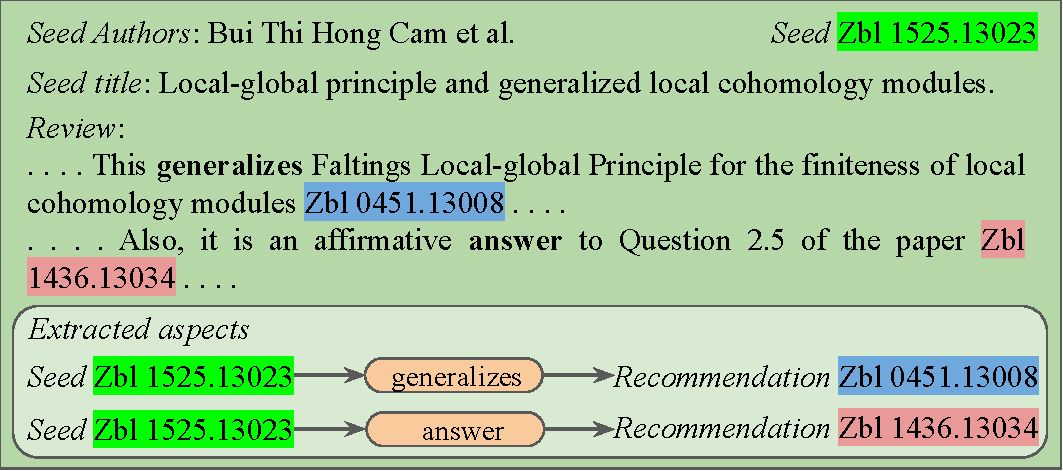
\includegraphics[width=0.48\textwidth]{images/aspect_SILVERst.pdf}
    \caption[An example seed BRE from zbMATH Open]{%
        An example seed BRE (Zbl 1525.13023~\cite{exSeedBRE})\protect\footnotemark[1]
        from zbMATH Open with potential recommendations 
        (Zbl 0451.13008\protect\footnotemark[2]~\cite{exRecmndBRE1}, 
        Zbl 1436.13034\protect\footnotemark[3]~\cite{exRecmndBRE2}) and extracted aspects 
        in the SilverRIM dataset.%
    }
    \label{fig:exampleSILVER}
\end{figure}
\footnotetext[1]{\url{https://zbmath.org/1525.13023}}
\footnotetext[2]{\url{https://zbmath.org/0451.13008}}
\footnotetext[3]{\url{https://zbmath.org/1436.13034}}

In zbMATH Open, reviewers often cite other works directly within the review texts they write (in-review citations).
A reviewer may cite a prior paper to highlight an important connection in a method, a shared motivation, or a result, among other reasons.
We consider these in-review citations as weak signals for recommendations.
Since recommendations in \textbf{GoldRiM} also show strong citation overlap, it is reasonable to treat in-review citations as recommendations.
When the cited works exist in zbMATH Open, reviewers include the respective ID (Zbl) to enable direct access.
These in-review citations, along with the sentences in which they appear, reveal the relationship between the citing and cited works, similar to the aspects identified in \textbf{GoldRiM}.
This helps us uncover additional aspects through which recommendations in mathematics may be related.
Figure~\ref{fig:exampleSILVER} shows an example zbMATH Open seed BRE with its in-review citations as potential recommendations.
The two aspects, \textit{generalizes} and \textit{answer}, in the example indicate distinct relationships between the recommendations and the seed paper.

As of October 2025, zbMATH Open contains 812,241 BREs with 1,286,410 in-review citations.
Manual extraction of in-review citations and their aspects across millions of BREs is infeasible.
Considering that obtaining a single review in zbMATH Open already requires several months\footnote{\url{https://zbmath.org/about/\#:~:text=Indexing\%20decisions\%22.-,Reviewing,-Published\%20items\%20are}}.
We expect a similar amount of time for manually constructing recommendations and aspects, as both require comparable expertise.
Therefore, we employ an LLM-based approach to automatically extract such relationships.
To obtain aspects, we utilize Qwen2.5-14B~\cite{qwen2025qwen25technicalreport} as it's the best-performing~\cite{koloveas2025can} few-shot model in the citation-intent prediction task on the SciCite~\cite{cohan2019structural} and ACL-LRC~\cite{Jurgens2018ACLARC} datasets.
On both datasets, Qwen2.5-14B was able to identify the relationship, such as \textit{Background}, \textit{Method}, or \textit{Result}, in which research papers are similar, with the highest accuracy among instruction LLMs.
Although LLM-based extractions are not as accurate as humans, annotations with prompts such as phrase extraction produce human-annotated-like data if not better than humans~\cite{horych-etal-2025-promises,tan-etal-2024-large,qin-etal-2023-chatgpt}.
Our objective here is not to evaluate the LLM, but to leverage it to efficiently generate weakly supervised relationships to understand how recommendations in mathematics are connected.
This allows us to construct a large-scale dataset with aspect-level explanations for recommendations.

We designed a concise few-shot prompt (Appendix~\ref{Appendix:prompt}) with three examples, as prior work indicates that larger prompts (e.g., 10 examples) reduce accuracy~\cite{koloveas2025can}. 
The model is asked to relationship in JSON format, enabling structured outputs even when multiple citations appear within a single review.
We passed 812,241 BREs through Qwen2.5-14B using the designed prompt and asked it to get the mentioned Zbl citation along with the aspect.
It worked correctly for 795,871 BREs, and for others, it gave either erroneous JSON, no aspect, or an invalid Zbl.  
It assigned 978,238 unique relationships (including stop words) as a different aspect\footnote{counted considering \textit{Extends} and \textit{Extends to} as a separate relationship.}) for 1,031,239 BRE pairs.
We apply the following quality check steps to obtain the final set of aspects.
First, \textbf{Normalization}, in which we stem and lemmatize extracted aspects using the Porter Stemmer, reducing them to a consistent set of 10,728 base forms.
For example, \textit{introduce}, \textit{introduced}, \textit{introduces}, \textit{introducing} becomes \textit{introduce}.
Second, \textbf{Filtering}, we manually inspected the normalized relationships having less than 1000 BREs to remove those that did not make sense due to probable LLM errors or absence of a potential single-word aspect in the review. 
Such relationships include \textit{due}, \textit{first}, \textit{conference}, \textit{see}, \textit{roll}, etc. 
This step yields 919,655 recommendations with 7,241 aspects for 745,264 BREs.

The top 20 aspects and their frequencies are shown in Figure~\ref{fig:SilverRIMwordFreq}, and their short description devised based on examples is in Appendix Table~\ref{tab:silverrim_aspects}.
The aspect with the most BREs, i.e., \textit{collect} represents\footnote{For example, \url{https://zbmath.org/1557.90300} mentions a reference to a conference collection \url{https://zbmath.org/1531.93014} at zbMATH Open.} a collection of lecture notes or conference proceedings, such as an entry at zbMATH Open.
The aspects are shared across many papers, which shows that common patterns of connections exist in recommendations.
Four of the \textbf{GoldRiM} aspects: \textit{Motiv}, \textit{Case}, \textit{Extend}, and \textit{Compare} also appear in \textbf{SilverRiM}, confirming the reliability of the LLM-based aspects extraction.
Three aspects: \textit{Applic}, \textit{Alternativ}, and \textit{Specialize} are unique to \textbf{GoldRiM}, suggesting finer-grained distinctions made by the expert reviewer that were not captured in \textbf{SilverRiM}.
However, these distinctions are related to similar categories in \textbf{SilverRiM}.
For example, the \textit{Alternativ} aspect in \textbf{GoldRiM}, which captures relationships between studies offering alternative approaches, is conceptually close to the \textit{studi} aspect in \textbf{SilverRiM}, where the reviewer expresses it as “study.”
We retain these distinctions for future qualitative analyses, as they may be useful in differentiating types of similarity. 
The additional aspects identified in \textbf{SilverRiM} confirm our understanding from \textbf{GoldRiM} that mathematical recommendations are connected through distinct aspects.
Moreover, they expand the number of identified aspects, revealing additional discrete ways in which recommendations are connected—through theoretical, logical, and conceptual relationships rather than simple textual or formulaic similarity.
These relationships allow us to model recommendations as being linked through multiple types of aspects.
Dataset characteristics are summarized in Table~\ref{tab:dataset_characteristics}, and the construction steps are freely available\footnote{\url{https://anonymous.4open.science/r/Aspect-Similarity-Math-BRE-Recsys-8098/}\label{gitlink}}. 

\begin{figure}
    \centering
    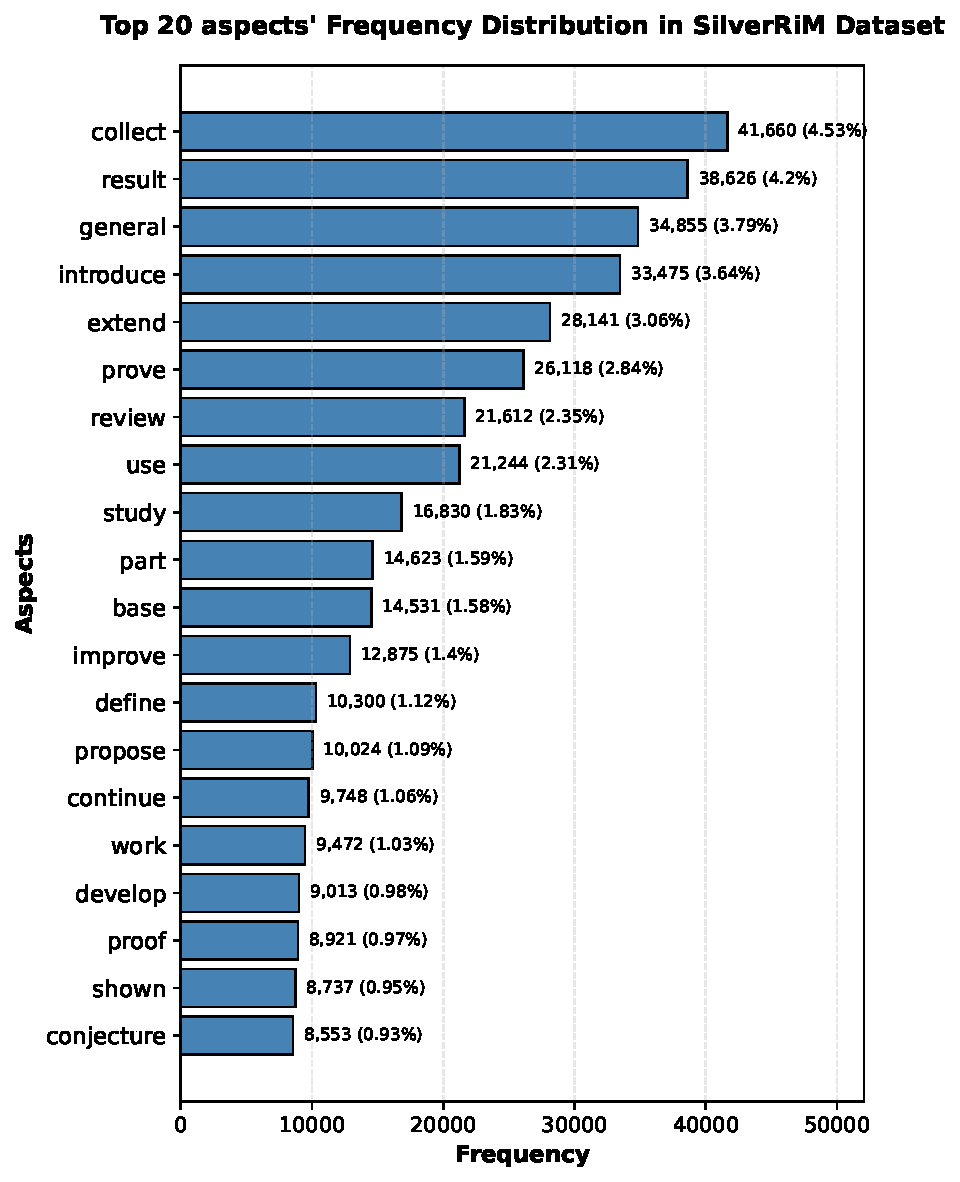
\includegraphics[width=0.5\textwidth]{images/silverrim_aspect_frequency_combined_halfway.pdf}
    \caption{Top 20 aspects' frequency distribution in the SilverRiM dataset.}
    \label{fig:SilverRIMwordFreq}
\end{figure}

\begin{table}[h]
\centering
\caption{Characteristics of GoldRiM and SilverRiM Datasets}
\label{tab:dataset_characteristics}
\begin{tabular}{lcc}
\hline
\textbf{Characteristic} & \textbf{GoldRIM} & \textbf{SilverRIM} \\
\hline
Total BRE Seeds & 80 & 745,264 \\
BRE Pairs (Recommendations) & 420 & 919,655 \\
Unique aspects & 7(for 100 pairs) & 7,241 \\
Recommendations per Seed & 5.25 & 1.23 \\
\hline
\end{tabular}
\end{table}

\section{Findings and discussion}

We established the \textbf{GoldRiM} and \textbf{SilverRiM} datasets, demonstrating that recommendations in mathematics are connected by aspect-level conceptual relationships rather than surface-level similarity.
To determine how recommendations are similar, we manually checked the text and citation overlap between pairs of recommendations obtained from an expert. 
We observed that articles without sharing most tokens or citations could be crucial, as it is logically assumed that they represent a natural flow of a work.
Furthermore, identifying similarities in zbMATH Open BREs is challenging, given that math is abstract and complex; in summary, one must understand their conceptual relationships, often through full-text documents.
Following the observations, we identified and annotated 7 aspects using an expert annotator and 7,241 aspects at scale using the LLM Qwen2.5-14B~\cite{qwen2025qwen25technicalreport}, which was enabled by the reviews in zbMATH Open.

Aspect-based similarity of research papers for recommendation has been studied before, as discussed in Section~\ref{sec:relatedWork}.
However, previous studies have primarily focused on papers from computer science, biomedical research, and mixed-domain research, missing mathematics.
In Table~\ref{tab:aspects}, we compare our identified and established mathematics-specific aspects with those used in previous studies on aspect-based similarity for recommendations, citation-intent prediction, and retrieval.
In our study, \textbf{we obtained aspects specific to mathematics}, such as \textit{Case}, \textit{Application}, \textit{Specialize}, to name a few, that are not available in existing datasets.
These aspects represent the connection of similar articles in mathematics as recommendations that are unique to the domain.
Additionally, there are shared aspects in mathematics and domains (Computer Science, Biomedicine) such as: \textit{Extend}, \textit{Alternative Approaches}, \textit{Comparisons}, and others.
While some of the \textbf{shared aspects are similar in meaning and explanation}, as commonly following the flow of research, such as \textit{Extend}, meaning extending a work, \textit{Compare}, meaning compares the work dealing with the same problem, etc. 
\textbf{There are aspects that share similar names but have different usage.}
For example, our identified aspect \textit{Alternative Approach} refers to an alternative proof, analysis, or conjecture presented in a research paper, while in existing datasets where it is identified, i.e., Modified AAN, the corresponding aspect includes all related work mentioned without specifying which one is actually the paper is actually based on or follows.
Further definition of aspects is available in Appendix~\ref{Appendix:aspects}.
We observe that the majority of aspects in existing work are motivated and derived from sections where citations are mentioned, but this is difficult in mathematics, as many times the paper is not structured in section fashion especially older math research paper dating to 1900s, as for some works, the only related work is a single paper, so authors only mention it briefly and then lets say carry on with the proof.
We also observed that aspects of mathematics are more logical than those based on experimentation, as noted in existing works.
Such logical aspects are \textit{Generalization}, \textit{Conjecture}, \textit{Theorem}, and \textit{Construct}, among others, showing the research connection. 
By using \textbf{GoldRiM} and \textbf{SilverRiM}, we establish evidence that indeed math research papers are connected in domain-specific aspects. 
% The aspects in \textbf{SilverRiM} and \textbf{GoldRiM} capture mathematics-specific conceptual relationships that are not present in existing datasets, and we have scale of 7 thousand aspects.
% For example, aspects such as \textit{Generalization}, \textit{Conjecture}, \textit{Theorem}, and \textit{Construct}, among others, identified in our datasets, are unique to mathematics and not present in previous studies.

These findings demonstrate that similar research papers in mathematics are connected in different aspects.
There are mathematics-specific aspects that are domain-dependent than seen in existing datasets.
Identified aspects and comparison highlights that mathematical research relationships are defined less by empirical evidence or shared datasets and more by logical, structural, and conceptual reasoning across problems, proofs, and methods..
This domain-specific nature underscores the importance of our newly established datasets for advancing recommendations in mathematics.
These findings suggest that modeling conceptual similarity, rather than surface-level textual or citation similarity, may be essential for building recommendation systems that accurately reflect similar research papers in mathematics.

\section{Conclusion}

We present the first study examining the recommendations in mathematics.
We studied similar research papers in mathematics as recommendations to establish two datasets, \textbf{GoldRiM} and \textbf{SilverRiM}.
We establish evidence to show that mathematical paper recommendations are defined not by surface-level similarity but by deep conceptual aspects.
% This finding calls for a paradigm shift in how scholarly recommender systems are designed for theoretical disciplines. 
Future work will leverage these datasets to develop aspect-aware embedding models, graph neural networks, and hybrid recommendation systems tuned for mathematical reasoning and expertise.
% \section{RQ2: How do existing systems perform? and qualitative analysis}

% doc1, doc2, aspectlabel 0 or 1, train model for each aspect, and then get similar candidates for each aspect by retrieving embeddings.
% For each aspect you need to train an embedding model, so it is infeasible to have 560 embedding models, with each model having to embed 5 million docs for retrieval. 

% \section{RQ3: trained GNN for reviewer-preferences based recommendations and qualitative analysis}

\section{Acknowledgments}

We utilized AI models, including ChatGPT, Claude, and Perplexity AI, to proofread, enhance grammar, and improve sentence clarity. 
Every sentence in the resulting text is checked by the authors, and citations are provided wherever available. 
We take full responsibility for the text in this manuscript.
%%
%% The next two lines define the bibliography style to be used, and
%% the bibliography file.
\bibliographystyle{ACM-Reference-Format}
\bibliography{main_}


\appendix

\section{Prompt used for extracting SilverRIM aspects}\label{Appendix:prompt}

\section*{Task Description}
You are tasked with extracting the relationship between a statement and its cited work (indicated by a Zbl reference number). Identify the key phrase that describes how the current work relates to each cited work.

Return your answer as a valid JSON object with the following structure:

\begin{lstlisting}[language=json]
{
  "citations": [
    {
      "zbl_number": "the Zbl reference number",
      "relationship": "the key phrase"
    }
  ]
}
\end{lstlisting}

\section*{Examples}

\subsection*{Example 1}

\textbf{Input:} ``For any integral arrangement $U$ and a chamber $\Delta$ the author constructs a local residue form $\omega_\Delta(U)$ and a pairing $\langle,\rangle$ such that for any $t\in\Delta$ one has $B_\Delta f(t)=\langle\omega_\Delta(U),f\exp(t)\rangle$. His constructions are essentially based on the notion of iterated residue of $U_C$-meromorphic functions where $U_C$ is the complexification of the arrangement $U$. The author underlines that his study of these sums was inspired by the works of E. Witten [Commun. Math. Phys. 141, 153-209 (1991; Zbl 0762.53063) and J. Geom. Phys. 9, 303-368 (1992; Zbl 0768.53042)].''

\textbf{Output:}
\begin{lstlisting}[language=json]
{
  "citations": [
    {
      "zbl_number": "Zbl 0762.53063",
      "relationship": "inspired"
    },
    {
      "zbl_number": "Zbl 0768.53042",
      "relationship": "inspired"
    }
  ]
}
\end{lstlisting}

\subsection*{Example 2}

\textbf{Input:} ``The authors investigates the natural question of the rationality of $f$. Previously, J. J. Duistermaat and W. van der Kallen [Indag. Math., New. Ser. 9, No. 2, 221–231 (1998; Zbl 0916.22007)] proved that if $I_\lambda(f_\sigma,\omega)\in C(\lambda)$ and $f$ is a proper non-constant morphism, then $I_\lambda(f_\sigma,\omega)=0$. Here, a necessary and sufficient condition for $I_\lambda(f_\sigma,\omega)$ to extend to a single-valued holomorphic function on the complement of a finite set in $P^1(\mathbb{C})$ is given. By a result of N. Nilsson [Ark. Mat. 5, 527–540 (1965; Zbl 0144.36302)] this is equivalent to the rationality of $I_\lambda(f_\sigma,\omega)$. Moreover, the criterion can be used to determine the set $\{\sigma\mid I_\lambda(f,\sigma,\omega)\in C(\lambda)\}$ from the pair $(f,\omega/df)$ when $X$ is a curve.''

\textbf{Output:}
\begin{lstlisting}[language=json]
{
  "citations": [
    {
      "zbl_number": "Zbl 0916.22007",
      "relationship": "proved"
    },
    {
      "zbl_number": "Zbl 0144.36302",
      "relationship": "result"
    }
  ]
}
\end{lstlisting}

\subsection*{Example 3}

\textbf{Input:} ``The paper under review was motivated by some questions on compact Lie groups raised by O. Mathieu [in: Algèbre non commutative, groupes quantiques et invariants. Sémin. Congr. 2, 263–279 (1995; Zbl 0889.22008)]. In the last section, the author gives a counterexample to Mathieu's second conjecture.''

\textbf{Output:}
\begin{lstlisting}[language=json]
{
  "citations": [
    {
      "zbl_number": "Zbl 0889.22008",
      "relationship": "motivated"
    }
  ]
}
\end{lstlisting}

\subsection*{Example 4}

\textbf{Input:} ``Now, strictly speaking the second category does not make sense at the present time since the semi-infinite flag manifold does not carry an algebro-geometric structure allowing a theory of perverse sheaves on it. The authors circumvent this problem by defining an ad-hoc category $\text{Perv}(\text{Fl}_{\infty/2})$; this approach was initiated in [M. Finkelberg, I. Mirkovic, Differential topology, infinite-dimensional Lie algebras, and applications. D. B. Fuchs 60th anniversary collection. Providence, RI: American Mathematical Society. Transl., Ser. 2, Am. Math. Soc. 194(44), 81–112 (1999; Zbl 1076.14512)]. The definition uses a geometric object introduced by Drinfeld and denoted $\overline{\text{Bun}}_{N^-}$. This object $\overline{\text{Bun}}_{N^-}$ classifies principal $G$-bundles on $X$ endowed with a possibly degenerate reduction to the maximal unipotent subgroup $N^-$; see [A. Braverman, M. Sanz-Solé, (ed.) et al., Proceedings of the international congress of mathematicians (ICM), Madrid, Spain, August 22–30, 2006. Volume II: Invited lectures. Zürich: European Mathematical Society (EMS), 1145–1170 (2006; Zbl 1118.22007)] for more details and references.''

\textbf{Output:}
\begin{lstlisting}[language=json]
{
  "citations": [
    {
      "zbl_number": "Zbl 1076.14512",
      "relationship": "initiated"
    },
    {
      "zbl_number": "Zbl 1118.22007",
      "relationship": "details"
    }
  ]
}
\end{lstlisting}

\section*{Test Case}

\textbf{Input:} ``About fifteen years ago, the physicist E. Verlinde proposed a stunning formula for the dimension of the space of conformal blocks within the Wess-Zumino-Witten model of conformal quantum field theory. Verlinde's formula involves certain rational trigonometric sums of highly complicated combinatorial structure, whose effective computation represents a real mathematical challenge. On the other hand, this formula turned out to have a close relationship to the geometry of the moduli spaces of flat connections over compact Riemann surfaces, and it was this spectacular, utmost striking discovery that opened the way to computing various intersection numbers in the enumerative geometry of such moduli spaces. The paper under review makes another step forward in this direction. Namely, in order to help to uncover the geometric information hidden in Verlinde's formula, the author derives a compact polynomial formula computing certain rational trigonometric sums occuring in this context. Building upon his earlier results on rational sums and Bernoulli polynomials corresponding to central hyperplane arrangements [A. Szenes, Int. Math. Res. Not. 1998, No. 18, 937-956 (1998; Zbl 0968.11015)], the author extends these investigations to affine hyperplane arrangements, obtains then a local formula for rational trigonomteric sums of ``Verlinde-type'', and compares his formula to a related result in the work of J.-M. Bismut and F. Labourie [Symplectic geometry and the Verlinde formulas, Surv. Differ. Geom., Suppl. J. Differ. Geom. 5, 97–311 (1999; Zbl 0997.53066)]. In fact, and as the author points out, one of the main goals of his paper under review is to prove the equality of the two formulas, which is achieved in great generality. Finally, the author's local sum formula is also related to the results of M. Brion and M. Vergne on vector partition functions [J. Am. Math. Soc. 10, 797–833 (1997; Zbl 0926.52016)]. However, this particular relationship is still in the process of closer inspection [A. Szenes and M. Vergne, Adv. Appl. Math. 30, 295–342 (2003; Zbl 1067.52014)]. No doubt, the paper under review is an important contribution to the current research on the combinatorics and geometry of the Verlinde formulas.''

\textbf{Expected Output:}
\begin{lstlisting}[language=json]
{
  "citations": [
    {
      "zbl_number": "Zbl 0968.11015",
      "relationship": "results"
    },
    {
      "zbl_number": "Zbl 0997.53066",
      "relationship": "compares"
    },
    {
      "zbl_number": "Zbl 0926.52016",
      "relationship": "related"
    },
    {
      "zbl_number": "Zbl 1067.52014",
      "relationship": "inspection"
    }
  ]
}
\end{lstlisting}

% Appendix: Aspect Definitions
\section*{Appendix A: Aspect Definitions}
\label{Appendix:aspects}

\begin{table*}[h]
\centering
\caption{GoldRiM Aspect Definitions}
\label{tab:goldrim_aspects}
\small
\begin{tabular}{p{2.5cm}p{12cm}}
\hline
\textbf{Aspect} & \textbf{Description} \\
\hline
Extend & extends results, theorems, or methods from the referenced paper to broader contexts, higher dimensions, or more general settings \\
\hline
Case & examines a specific case, special instance, or particular example of concepts presented \\
\hline
Applic & applies methods, theorems, or techniques from the seed paper to solve problems in different mathematical areas or practical domains \\
\hline
Alternativ & presents an alternative approach, different proof method, or competing technique for addressing the same mathematical problem or question \\
\hline
Motiv & provides motivation, context, or foundational ideas that inspired or led to the work \\
\hline
Specialize & focuses on a more specialized or restricted version of the general framework presented \\
\hline
Compare & compares, contrasts, or evaluates different methods, results, or approaches discussed in the seed paper \\
\hline
\end{tabular}
\end{table*}

\begin{table*}[h]
\centering
\caption{SilverRiM Top 20 Aspect Definitions}
\label{tab:silverrim_aspects}
\small
\begin{tabular}{p{2.5cm}p{12cm}}
\hline
\textbf{Aspect} & \textbf{Description} \\
\hline
introduc & used concepts, definitions, objects, or frameworks that are introduced \\
\hline
gener & generalizes results, methods, or structures from more specific or restrictive cases \\
\hline
extend & extends prior results, theorems, or techniques to new settings, dimensions, or conditions \\
\hline
prove & proves theorems, lemmas, or conjectures that are cited or built upon \\
\hline
studi & studies, investigates, or analyzes mathematical objects, phenomena, or structures \\
\hline
part & forms part of a series, related body of work, part 1 or two of the same works or larger research program \\
\hline
propos & proposes new methods, algorithms, conjectures, or theoretical frameworks based on referenced paper \\
\hline
continu & continues research, extends earlier work, or builds upon previous investigations \\
\hline
improv & improves existing results, bounds, estimates, or methods \\
\hline
discuss & discusses topics, questions, or implications that are also addressed in the referenced paper \\
\hline
defin & refrenced papers defines mathematical objects, structures, or concepts that are used in the seed paper \\
\hline
develop & develops theory, methods, or tools that are applied or mentioned \\
\hline
deriv & derives formulas, equations, identities, or results that appear in or relate \\
\hline
correct & corrects errors, refines arguments, or addresses issues from earlier work discussed in the seed paper \\
\hline
investig & investigates properties, behaviors, or characteristics of mathematical structures also studied in the seed paper \\
\hline
conjectur & poses conjectures, open problems, or questions that are addressed or mentioned \\
\hline
translat & translates concepts, results, or methods between different mathematical languages, frameworks, or areas of study \\
\hline
origin & presents original work that serves as a foundation or starting point for developments \\
\hline
question & raises questions, problems, or research directions that are explored or answered \\
\hline
establish & establishes fundamental results, frameworks, or theories that underpin work presented \\
\hline
\end{tabular}
\end{table*}

\noindent \textbf{Note:} These aspect definitions were derived from analysis of in-review citations in zbMATH Open reviews. Aspects describe the relationship between a seed paper and its recommended related work, indicating why the recommendation is relevant to readers of the seed paper.

% \begin{table*}
% \centering
% \small
% \begin{tabular}{l|c:c:c:c:c|c:c:c:c:c}
% \hline
% \multicolumn{1}{l|}{Dataset$\rightarrow$} & \multicolumn{5}{c|}{SilverRiM} & \multicolumn{5}{c}{GoldRiM} \\
% \hline
% Model $\downarrow$ & \textbf{P@3} & \textbf{P@5} & \textbf{R@10} & \textbf{MRR} & \textbf{nDCG} & \textbf{P@3} & \textbf{P@5} & \textbf{R@10} & \textbf{MRR} & \textbf{nDCG}\\
% \hline
% SPECTER (Semantic Scholar) & 0.020 & 0.016 & 0.067 & 0.038 & 0.032 & 0.029 & 0.023 & 0.050 & 0.111 & 0.030\\
% DPR & 0.045 & 0.027 & 0.117 & 0.089 & 0.072 & 0.046 & 0.030 & 0.056 & 0.112 & 0.042 \\
% QWEN-2.5-MATH\_LLM2Vec  & 0.042 & 0.030 & 0.126 & 0.103 & 0.086 & 0.050 & 0.043 & 0.048 & 0.100 & 0.049\\
% % Approach0 & 0.050 & 0.030 & 0.140 & 0.180 &  0.140 & 0.042 & 0.025 & 0.063 & 0.063 & 0.048\\
% \hline
% \end{tabular}
% \caption{Performance of baseline models for k recommendation generation}
% \label{tab:baselne_zbRec}
% \end{table*}

\end{document}
\endinput
%%
%% End of file `sample-sigconf.tex'.
